\documentclass[12pt]{article}

% Packages
\usepackage{amsmath}
\usepackage{amssymb}
\usepackage{amsthm}
\usepackage{geometry}
\usepackage{setspace}
\usepackage{xcolor}
\usepackage{enumitem}
\usepackage{graphicx}
\usepackage{listings}
\usepackage{xcolor}
\usepackage{changepage}

% Custom colors for code highlighting
\definecolor{codegreen}{rgb}{0,0.6,0}
\definecolor{codegray}{rgb}{0.5,0.5,0.5}
\definecolor{codepurple}{rgb}{0.58,0,0.82}
\definecolor{backcolour}{rgb}{0.95,0.95,0.92}

% Style for Python code
\lstset{
    language=Python,
    backgroundcolor=\color{backcolour},
    commentstyle=\color{codegreen},
    keywordstyle=\color{magenta},
    numberstyle=\tiny\color{codegray},
    stringstyle=\color{codepurple},
    basicstyle=\ttfamily\small,
    breakatwhitespace=false,
    breaklines=true,
    captionpos=b,
    keepspaces=true,
    numbers=left,
    numbersep=5pt,
    showspaces=false,
    showstringspaces=false,
    showtabs=false,
    tabsize=2
}

% Define theorem, definition, and proof environments
\newtheorem{theorem}{Theorem}
\newtheorem{definition}{Definition}
\newtheorem{lemma}{Lemma}
\newtheorem{corollary}{Corollary}
\newtheorem{proposition}{Proposition}
\newtheorem{example}{Example}
\newtheorem{remark}{Remark}

% Set up the page margins
\geometry{left=0.5in,right=0.5in,top=0.5in,bottom=0.75in}

\begin{document}
\doublespacing % Use this command for double spacing

\title{HW-06}
\author{Abraham J. Reines}
\date{\today}
\maketitle

\section*{Introduction 6.1.16}
In this assignment, we delve into the intricacies of set theory by examining the relationships between three distinct sets. Through the application of intersection, union, and difference operations, we uncover the nuanced dynamics of these sets.

\section*{Problem Statement}
Consider the sets \( A = \{ a, b, c \} \), \( B = \{ b, c, d \} \), and \( C = \{ b, c, e \} \). The tasks are to:
\begin{enumerate}[label=\alph*.]
    \item Illustrate the relationships between these sets using a Venn diagram.
    \item Determine the composition of specific combinations of these sets and identify any equivalences:
    \begin{enumerate}[label=\arabic*.]
        \item \( A \cap (B \cup C) \)
        \item \( (A \cap B) \cup C \)
        \item \( (A \cap B) \cup (A \cap C) \)
    \end{enumerate}
    \item Evaluate the results of different set difference operations and ascertain their equality:
    \begin{enumerate}[label=\arabic*.]
        \item \( (A - B) - C \)
        \item \( A - (B - C) \)
    \end{enumerate}
\end{enumerate}

\section*{Solution}
\subsection*{Venn Diagram}
Refer to the Venn diagram for a visual representation of the sets \( A \), \( B \), and \( C \).

\begin{figure}[h]
\centering
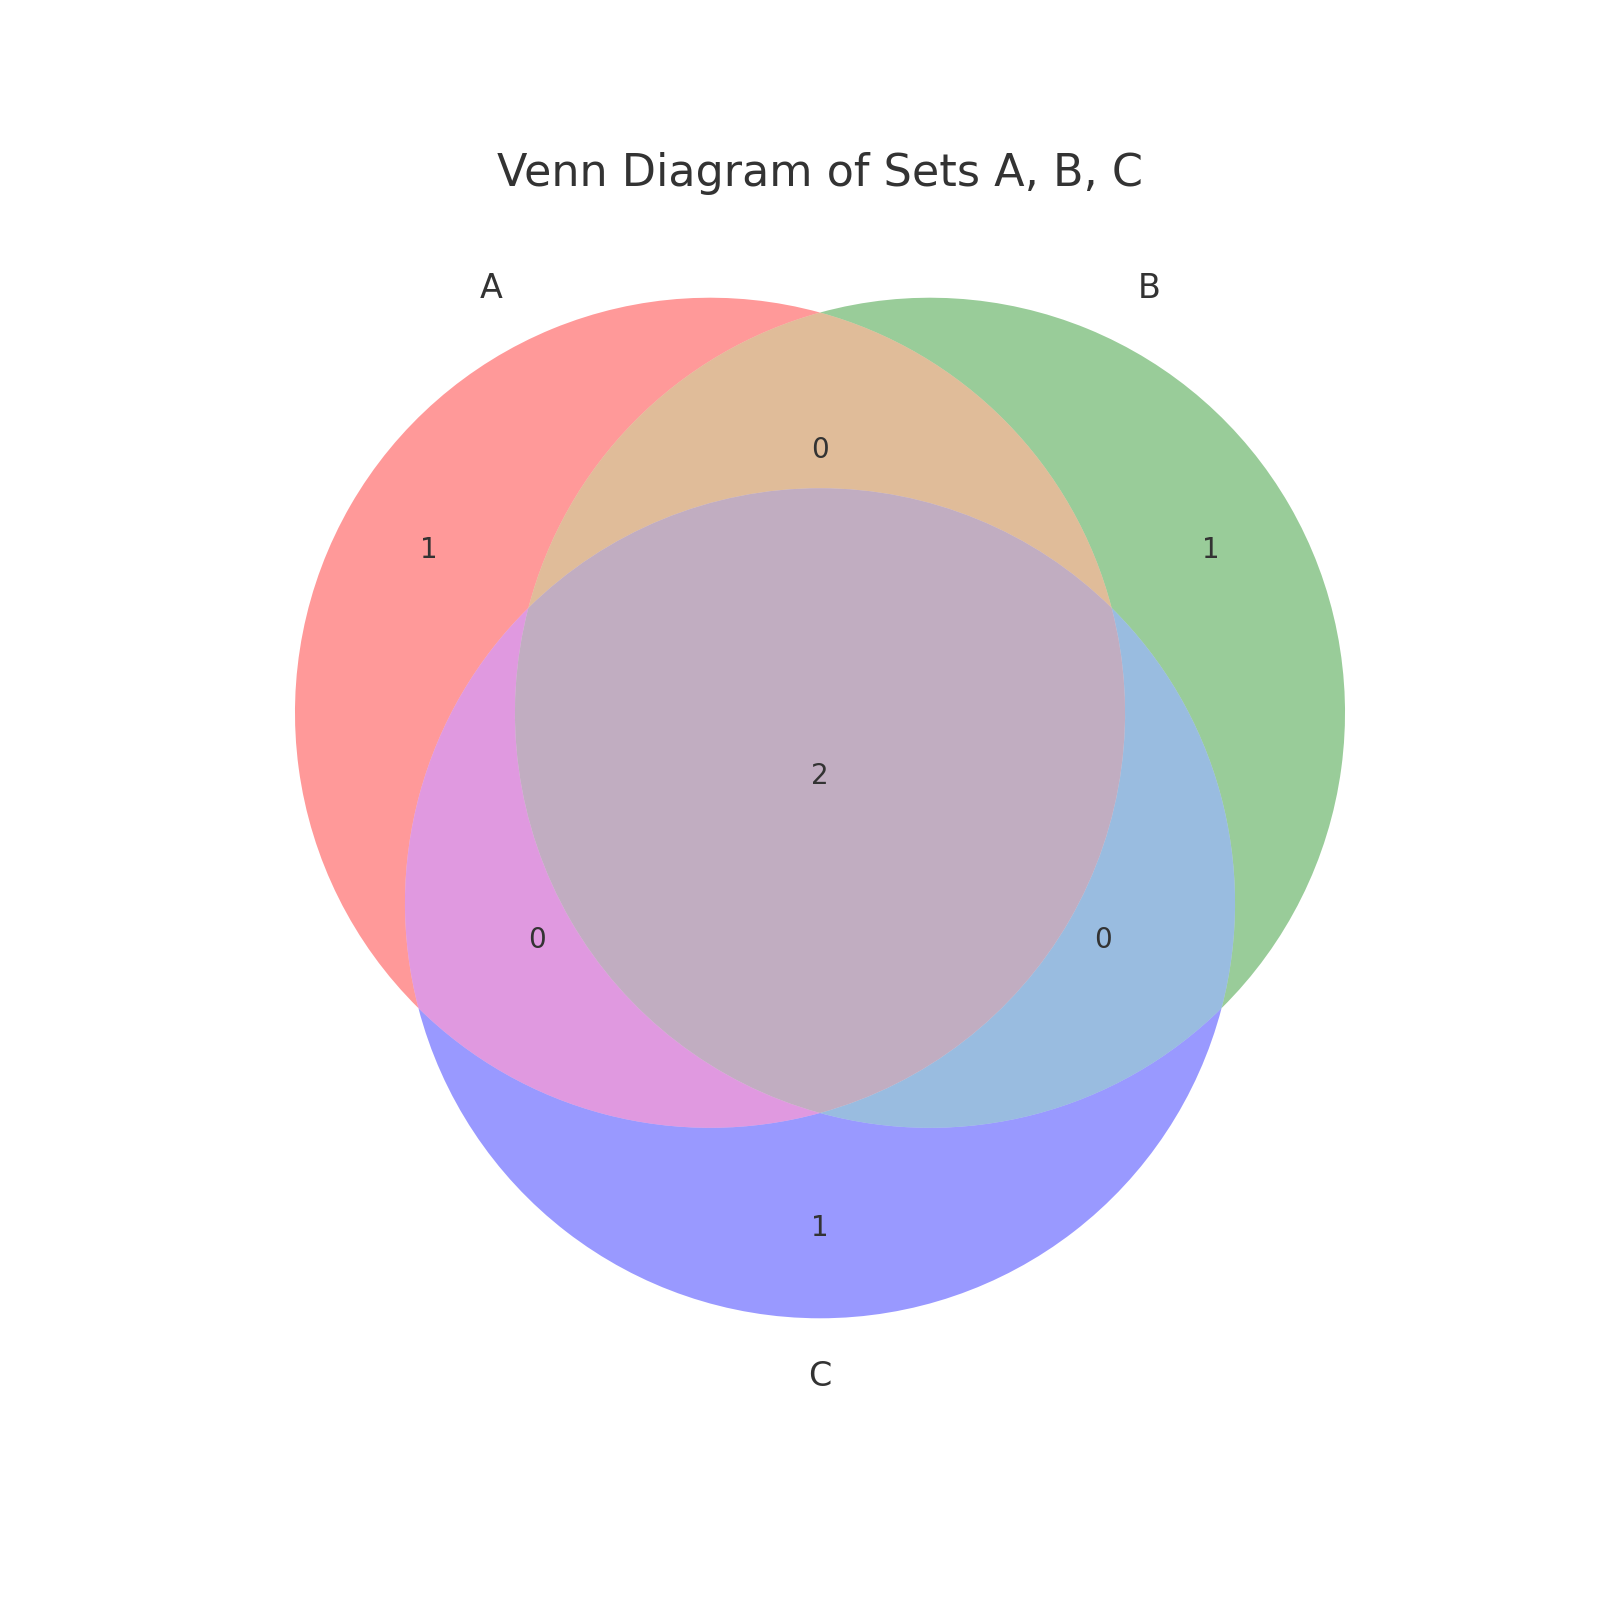
\includegraphics[width=0.75\textwidth]{venn_diagram.png} % Adjust the filename as necessary
\caption{Venn Diagram of Sets A, B, C*}
\end{figure}

\newpage
\textbf{*Code for Figure 1:} To show logic behind the formulation of the Venn Diagram.
\begin{lstlisting}
import matplotlib.pyplot as plt
import matplotlib_venn as venn

# Define the sets
A = set(['a', 'b', 'c'])
B = set(['b', 'c', 'd'])
C = set(['b', 'c', 'e'])

# Create a Venn diagram
plt.figure(figsize=(8, 8))
venn_diagram = venn.venn3([A, B, C], ('A', 'B', 'C'))

# Show the Venn diagram
plt.title("Venn Diagram of Sets A, B, C")
plt.show()
\end{lstlisting}

\subsection*{Part b: Calculations of Intersection and Union}
\begin{itemize}
    \item \( A \cap (B \cup C) \): We calculate the union of \( B \) and \( C \) first, then find the intersection with \( A \).
    \begin{align*}
        B \cup C &= \{ b, c, d \} \cup \{ b, c, e \} = \{ b, c, d, e \} \\
        A \cap (B \cup C) &= \{ a, b, c \} \cap \{ b, c, d, e \} = \{ b, c \}
    \end{align*}
    \item \( (A \cap B) \cup C \): Here, we calculate the intersection of \( A \) and \( B \), then unite it with \( C \).
    \begin{align*}
        A \cap B &= \{ a, b, c \} \cap \{ b, c, d \} = \{ b, c \} \\
        (A \cap B) \cup C &= \{ b, c \} \cup \{ b, c, e \} = \{ b, c, e \}
    \end{align*}
    \item \( (A \cap B) \cup (A \cap C) \): We calculate both intersections and then their union.
    \begin{align*}
        A \cap B &= \{ a, b, c \} \cap \{ b, c, d \} = \{ b, c \} \\
        A \cap C &= \{ a, b, c \} \cap \{ b, c, e \} = \{ b, c \} \\
        (A \cap B) \cup (A \cap C) &= \{ b, c \} \cup \{ b, c \} = \{ b, c \}
    \end{align*}
\end{itemize}

\subsection*{Part c: Calculations of Set Difference}
\begin{itemize}
    \item \( (A - B) - C \): We first subtract \( B \) from \( A \) and then subtract \( C \) from the result.
    \begin{align*}
        A - B &= \{ a, b, c \} - \{ b, c, d \} = \{ a \} \\
        (A - B) - C &= \{ a \} - \{ b, c, e \} = \{ a \}
    \end{align*}
    \item \( A - (B - C) \): Here, we subtract \( B - C \) from \( A \).
    \begin{align*}
        B - C &= \{ b, c, d \} - \{ b, c, e \} = \{ d \} \\
        A - (B - C) &= \{ a, b, c \} - \{ d \} = \{ a, b, c \}
    \end{align*}
\end{itemize}

\section*{Conclusion 6.1.16}

The exercises demonstrated the importance of the order of operations in set theory. While some intersections and unions resulted in equal sets, the differences in sets showed distinct outcomes. This underlines the significance of precise operations in mathematical set theory.

\section*{6.1.32}

Let $X = \{a, b\}$ and $Y = \{x, y\}$. The Cartesian product $X \times Y$ is defined as:

\[ X \times Y = \{(a, x), (a, y), (b, x), (b, y)\} \]

The power set $P(X \times Y)$, which is the set of all subsets of $X \times Y$, includes:

\begin{enumerate}
    \item $\emptyset$ (the empty set)
    \item $\{(a, x)\}$
    \item $\{(a, y)\}$
    \item $\{(b, x)\}$
    \item $\{(b, y)\}$
    \item $\{(a, x), (a, y)\}$
    \item $\{(a, x), (b, x)\}$
    \item $\{(a, x), (b, y)\}$
    \item $\{(a, y), (b, x)\}$
    \item $\{(a, y), (b, y)\}$
    \item $\{(b, x), (b, y)\}$
    \item $\{(a, x), (a, y), (b, x)\}$
    \item $\{(a, x), (a, y), (b, y)\}$
    \item $\{(a, x), (b, x), (b, y)\}$
    \item $\{(a, y), (b, x), (b, y)\}$
    \item $\{(a, x), (a, y), (b, x), (b, y)\}$ (the set itself)
\end{enumerate}

In summary, the Cartesian product of two sets $X$ and $Y$, denoted as $X \times Y$, results in a set comprising all possible ordered pairs formed by taking the first element from set $X$ and the second from set $Y$. The power set $P(X \times Y)$ includes all possible subsets of the Cartesian product, encompassing everything from the empty set to the set itself. For the sets $X = \{a, b\}$ and $Y = \{x, y\}$, the power set contains 16 distinct subsets, demonstrating the exponential growth of the power set relative to the size of the original sets. This concept is fundamental in set theory and has various applications in mathematics, computer science, and logic.

\section*{Objective 6.2.35}
\begin{theorem}To rigorously demonstrate for any sets \( A, B, C, \) and \( D \) within a universal set, if \( A \cap C = \emptyset \), then it necessarily follows \( (A \times B) \cap (C \times D) = \emptyset \).\end{theorem}

\section*{Method}
The proof will be conducted via the method of contradiction.

\section*{Proof}\begin{proof}
Let \( A, B, C, \) and \( D \) be arbitrary sets with the condition \( A \cap C = \emptyset \). We aim to establish under these conditions, \( (A \times B) \cap (C \times D) = \emptyset \).

Suppose, for the sake of contradiction, \( (A \times B) \cap (C \times D) \neq \emptyset \). Let \( (x, y) \) be an element in this intersection. By the nature of intersection, \( (x, y) \) belongs to both \( A \times B \) and \( C \times D \). Consequently, by the definition of Cartesian product, \( x \in A \) and \( y \in B \), and simultaneously \( x \in C \) and \( y \in D \).

However, this inference leads to a contradiction. The initial condition \( A \cap C = \emptyset \) dictates there are no common elements between sets \( A \) and \( C \). The existence of \( x \) in both \( A \) and \( C \) contravenes this condition.

Therefore, the assumption \( (A \times B) \cap (C \times D) \neq \emptyset \) must be false. It follows unequivocally \( (A \times B) \cap (C \times D) = \emptyset \) for any sets \( A, B, C, \) and \( D \) satisfying \( A \cap C = \emptyset \).
\end{proof}

\section*{Conclusion}
Through a deterministic approach utilizing the contradiction method, we have established the truth of the stated relationship between the intersections of sets and their Cartesian products. This conclusion aligns with fundamental principles of set theory within the realm of discrete mathematics.

\end{document}
